\section{Implementation}
\label{sec:implementation}
% ALL

Ontoqa has been realized as a Java\footnote{Oracle Java SE 8} web and standalone application, packaged with Maven.
%
Ontoqa can be executed both as a standalone application and as a web application.
%
All functionalities has been tested carefully against 224 total unit tests.

Ontoqa leverages some well known technologies. Here we present them, giving an idea about how they have been used in our implementation. The reader may refer to the open source code of the project and the corresponding Javadocs to get into the implementation details.


\begin{itemize}
	\item[Ontology] INSERT HERE
	
	\item[Lexicon] The lexical information about ontology is reported in Java by using the APIs provided by the "Semantic Computing Group @ Bielefeld University". The APIs allow the representation of the lemon model in java and the use of lexinfo for generating grammar. The library was manipulated to shape the following lemon properties: 
	\begin{itemize}
		\item Recognition of entries of composite words
		\item Tense and number of different forms of entry 
	\end{itemize}	
Finally, where necessary, a parsing of meaningful terms extracted from paths has been implemented.
The library provided has been to retrieve the ontology represented by the Lemon model from the RDF file and to get a list of Lexical Entry consisting of the most relevant properties shown in the figure.

	\item[I/O] we used the Jackson core library and data-binding modules to implement data representation in JSON and YAML format.
	
	\item[CLI] we used Apache CLI to implement options and argument parsing for the command line interface.
	
	\item[Web UI] we used AngularJS, JQuery and JavaScript for navigation logic and HTML5 and Bootstrap for the page style.
	
	\item[Web Service] we used Spring Framework and Spring MVC to implement the REST service interface.
	
	\item[Logging] we used SLF4J to implement logging ayer as facade, and Logback as the underlying logging framework.
	
	\item[Development] we used Lombok to implement bean constructors, getter/setters, thus minimizing code redundancy.
	
	\item[Testing] we used JUnit4 to implement unit testing suites.
\end{itemize}

\begin{figure}[H]
   \centering
    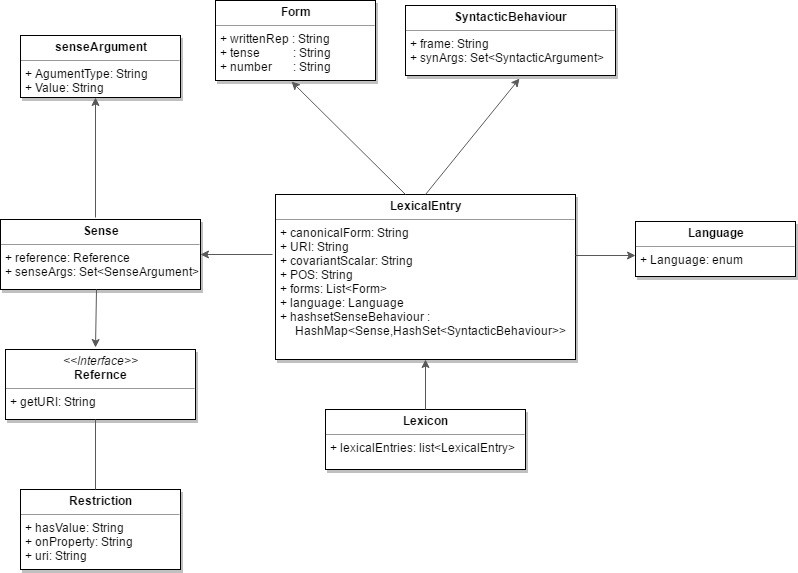
\includegraphics[scale=0.5]{./fig/lemon}
     \caption{Lemon Library}
    \label{fig: lemon}
\end{figure}

